\begin{textblock*}{\posterboxwidth}(0cm,0cm)
\centering%
\textbf{Main loop of the multiobjective evolutionary algorithm}\\[.5em]

\def\figscale{.5}
\def\figfontsize{\footnotesize}

\newcommand\pmabox[1]{%
\scalebox{\figscale}{%
\begin{tikzpicture}[font=\figfontsize]
\input{vector/StagesPMA_#1}
\draw (7,1.5) node[font=\normalsize,draw,circle] {#1};
\end{tikzpicture}}%
}

\newcommand\circled[1]{%
\raisebox{-.5em}{\tikz \draw (0,0) node[circle,draw] {#1};}%
}

\begin{tabular}{ccc}
\hspace{1em}\parbox[b]{4cm}{%
\small%
1. Choose a direction\\
2. Choose parents\\
3. Recombine\\
4. Do local search\\
5. Update Pareto set\\
\vspace*{1.5ex}
}&\pmabox{1}&\pmabox{2}\\
\pmabox{3}&\pmabox{4}&\pmabox{5}
\end{tabular}
\end{textblock*}

\begin{textblock*}{\posterboxwidth / 100 * 55 - 2ex}(\posterboxwidth / 100 * 45 + 2ex,\posterboxheight /4)
\centering%
\textbf{Achievement scalarizing functions}\\[.5em]

\scalebox{.5}{%
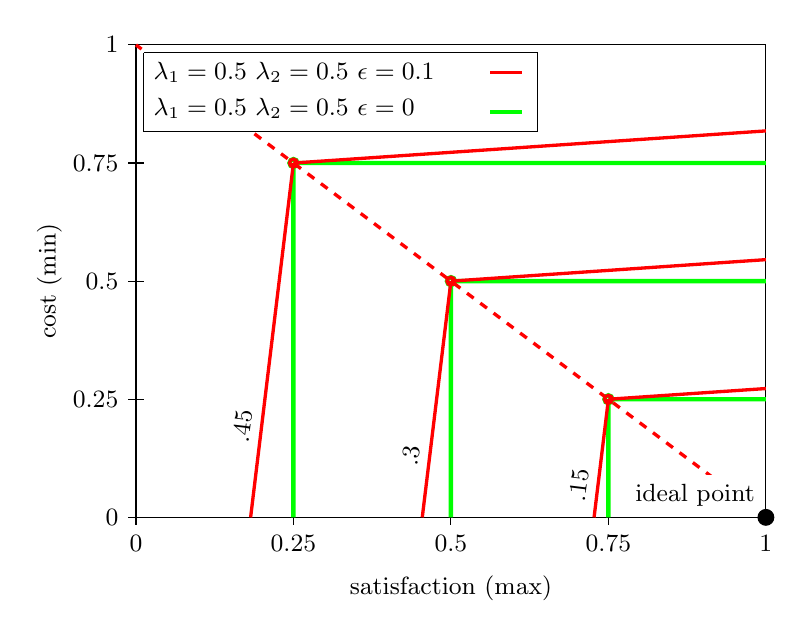
\begin{tikzpicture}[font=\small]
	% The axes
	\draw (0, 0) -- (8, 0) -- (8, 6) -- (0, 6) -- (0, 0);
	% Description of the axes
	\draw (4, -0.9) node[anchor=center] {satisfaction (max)};
	\draw [rotate=90] (3, +1.1) node[anchor=center, rotate=90] {cost (min)};
	% Ticks on the horizontal axis
	\foreach \x / \xtext in {0 / 0, 2 / 0.25, 4 / 0.5, 6 / 0.75, 8 / 1}
		\draw (\x cm, 0.1cm) -- (\x cm, -0.1cm) node[anchor=north]{\xtext};
	% Ticks on the vertical axis
	\foreach \y / \ytext in {0 / 0, 1.5/ 0.25, 3 / 0.5, 4.5 / 0.75, 6 / 1}
		\draw (-0.1cm, \y cm) node[anchor=east]{\ytext} -- (0.1cm, \y cm);
	% The related Tchebycheff weighted scalarizing function
	\begin{scope}[ultra thick, green]
	\draw (6, 0) -- node[near start, above, sloped, black]{} (6, 1.5) ++(0, 0) circle (0.05cm) -- (8, 1.5);
	\draw (4, 0) -- node[near start, above, sloped, black]{} (4, 3) ++(0, 0) circle (0.05cm) -- (8, 3);
	\draw (2, 0) -- node[near start, above, sloped, black]{} (2, 4.5) ++(0, 0) circle (0.05cm) -- (8, 4.5);
	\end{scope}
	% The achievement weighted scalarizing function
	\begin{scope}[very thick, red]
	\draw (5.818, 0) -- node[near start, above, sloped, black]{.15} (6, 1.5) ++(0, 0) circle (0.05cm) -- (8, 1.636);
	\draw (3.636, 0) -- node[near start, above, sloped, black]{.3} (4, 3) ++(0, 0) circle (0.05cm) -- (8, 3.273);
	\draw (1.456, 0) -- node[near start, above, sloped, black]{.45} (2, 4.5) ++(0, 0) circle (0.05cm) -- (8, 4.908);
		% the line through vertices
	\draw[dashed] (8, 0) -- (0, 6);
	\end{scope}
	% Legend
	\filldraw[fill=white,draw=black] (0.1, 5.9) -- (5.1, 5.9) -- (5.1, 4.9) -- (0.1, 4.9) -- (0.1, 5.9); % the boundary
	\draw (0.1, 5.9) node[anchor=north west] {$\lambda_1=0.5\ \lambda_2=0.5\ \epsilon=0.1$}; % first function text
	\draw[very thick, red] (4.5, 5.65) -- ++(0.4, 0); % first function line
	\draw (0.1, 5.45) node[anchor=north west] {$\lambda_1=0.5\ \lambda_2=0.5\ \epsilon=0$}; % second function text
	\draw[ultra thick, green] (4.5, 5.15) -- ++(0.4, 0); % second function line
	% The ideal point
	\draw (8, 0) node [above left=.5pt, fill=white] {ideal point};
	\filldraw[fill=black] (8, 0) circle (0.1cm);

\end{tikzpicture}}\\[1em]

\textbf{Local search: exchange of two customers}\\
\includegraphics[width=\posterboxwidth / 100 * 55 - 5ex]{bitmap/customerExchangeExample}\\[1em]

\textbf{Local search: relocation of a customer}\\
\includegraphics[width=\posterboxwidth / 100 * 55 - 5ex]{bitmap/customerRelocateExample}\\[1em]

\textbf{Route-based crossover}\\
\includegraphics[width=\posterboxwidth / 100 * 55 - 5ex]{bitmap/CEPXExample}\\[1em]

\textbf{Common edges preserving crossover}\\
\includegraphics[width=\posterboxwidth / 100 * 55 - 5ex]{bitmap/RBXExample}\\[1em]
\end{textblock*}